\begin{frame}
\frametitle{Linux - Motivation}

\begin{tabular}{cl}
	\begin{tabular}{c}
		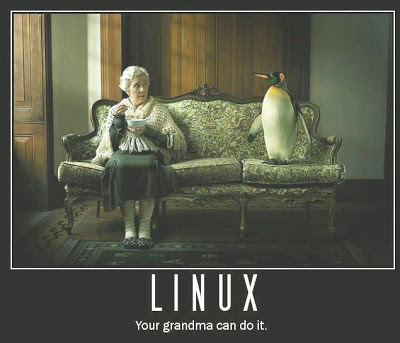
\includegraphics[scale=0.4]{resources/grandmaLinux.jpg}
	\end{tabular}
	& \begin{tabular}{l}
		\parbox{0.5\textwidth}{\begin{itemize}
				\item Linux ist überall
				\begin{itemize}
					\item Server
					\item Heimrechner
					\item Smartphone
				\end{itemize}
				%https://2.bp.blogspot.com/_UqUwVPikChs/TFq5scy4dVI/AAAAAAAAOiM/tDuYjZGTSgY/s1600/GrandmaLinux.jpg
		\end{itemize}}
	\end{tabular}
	
\end{tabular}
\end{frame}

\begin{frame}
\frametitle{Was ist Linux?}
\begin{figure}

\includegraphics[scale=0.17]{resources/tux.png}
\end{figure}
\begin{itemize}
\item Free and Open-Source Betriebssystem
\item Projekt wird unterstützt von Unternehmen, Non-Profit-Organisationen und vielen Freiwilligen
\item Basiert auf dem Linux-Kernel
\item Linux-Distribution fasst Kernel und unterschiedliche Software zusammen
\end{itemize}
\end{frame}

\subsection{Distros}
\begin{frame}{Distributionen}
\note{Mint, OpenSuse, ubuntu, Fedora\\}
\note{alle direkt benutzbar}
\begin{columns}
\begin{column}{0.5\textwidth}
	\begin{figure}
		
\includegraphics[width=0.9\textwidth]{resources/640px-Linux_Mint_logo_and_wordmark}
		%https://de.wikipedia.org/wiki/Linux_Mint#/media/File:Linux_Mint_logo_and_wordmark.svg
	\end{figure}
	
	\begin{figure}
		
\includegraphics[width=0.8\textwidth]{resources/640px-OpenSUSE_Logo}
		%https://de.wikipedia.org/wiki/OpenSUSE#/media/File:OpenSUSE_Logo.svg
	\end{figure}
	
\end{column}
\begin{column}{0.5\textwidth}
	
	\begin{figure}
		
\includegraphics[width=0.9\textwidth]{resources/640px-Ubuntu_logo}
		%https://de.wikipedia.org/wiki/Ubuntu#/media/File:Ubuntu_logo.svg
	\end{figure}
	
	\begin{figure}
		
\includegraphics[width=0.9\textwidth]{resources/640px-Fedora_logo_and_wordmark}
		%https://de.wikipedia.org/wiki/Fedora_%28Linux-Distribution%29#/media/File:Fedora_logo_and_wordmark.svg
	\end{figure}
	
\end{column}
\end{columns}
\end{frame}

\subsection{Oberflächen}
\begin{frame}{Oberflächen}{Gnome}
\note{komplett tauschbare Oberflächen/DEs}
\note{Gnome3\\}
\begin{figure}
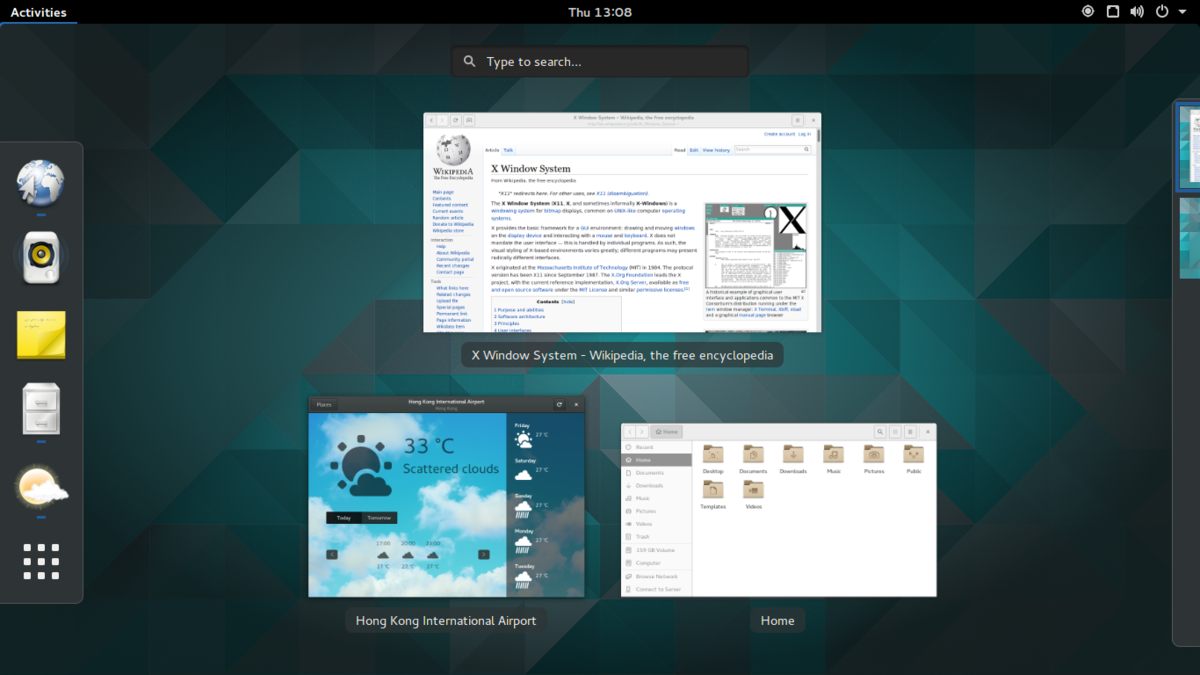
\includegraphics[height=0.6\textheight]{resources/1200px-GNOME_Shell.png}
%https://de.wikipedia.org/wiki/Gnome-Shell#/media/File:GNOME_Shell.png
\end{figure}

\end{frame}

\begin{frame}{Oberflächen}{KDE}

\note{KDE/Plasma\\}
\begin{figure}
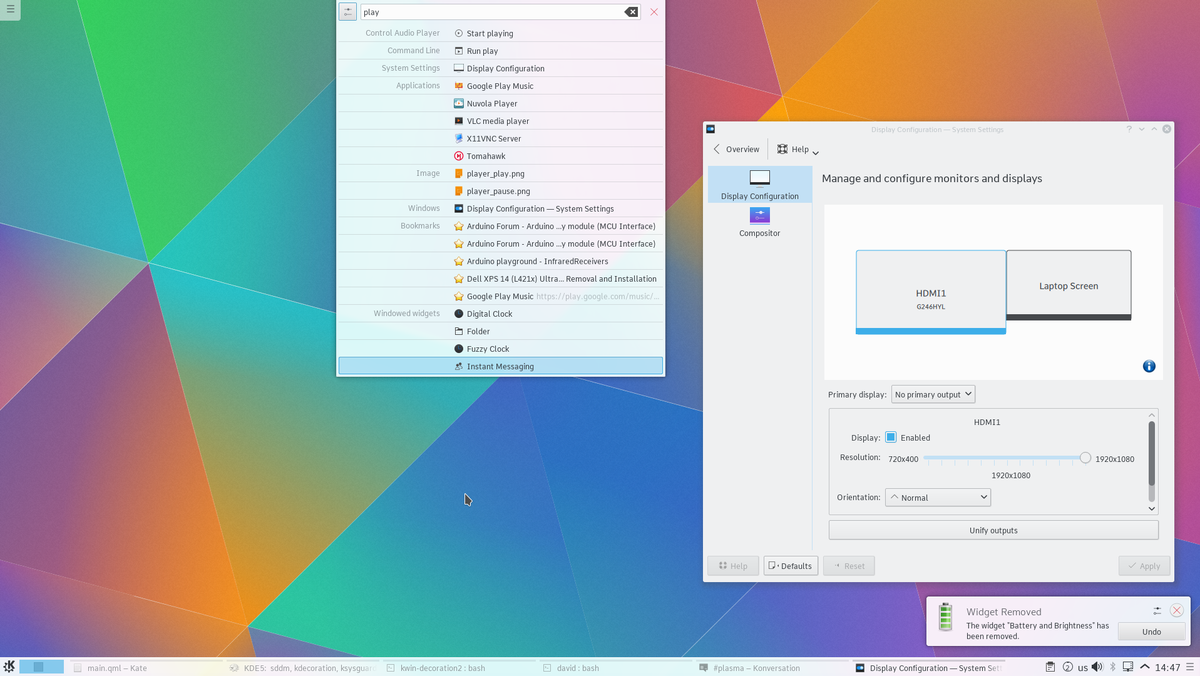
\includegraphics[height=0.6\textheight]{resources/1200px-Kscreen-krunner.png}
%https://en.wikipedia.org/wiki/KDE_Plasma_5#/media/File:Kscreen-krunner.png
\end{figure}


\end{frame}

\begin{frame}{Oberflächen}{Cinnamon}
\note{Cinnamon/Mint\\}
\begin{figure}
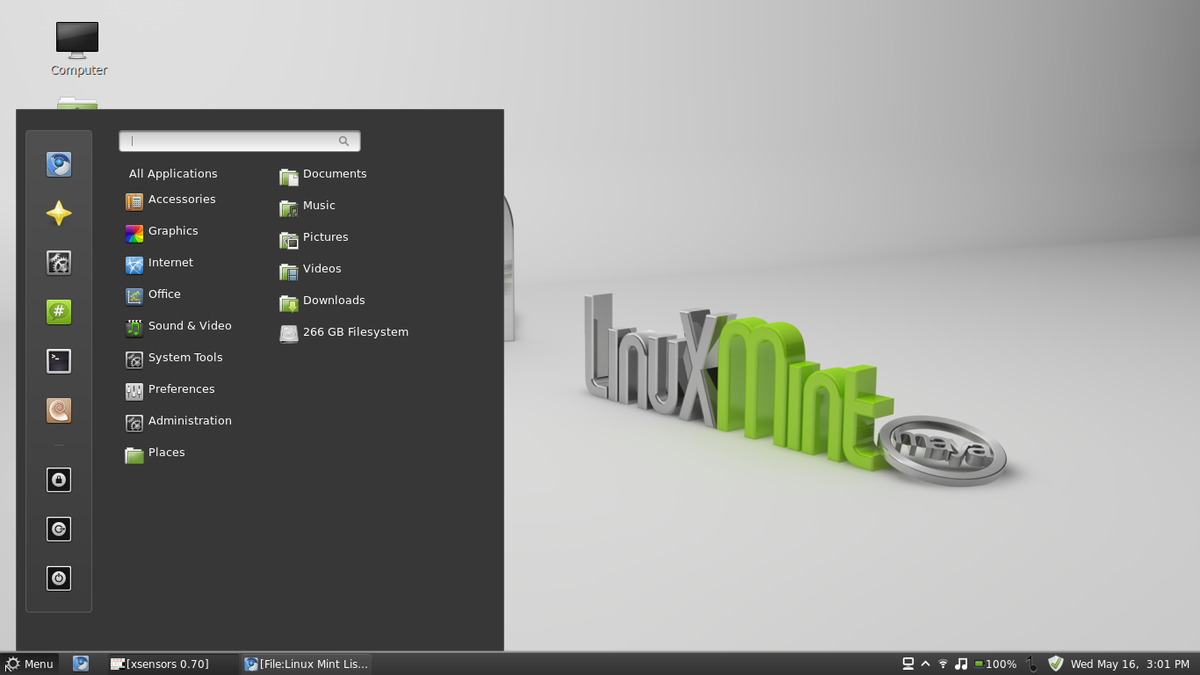
\includegraphics[height=0.6\textheight]{resources/1200px-Linux_Mint.png}
%https://de.wikipedia.org/wiki/Cinnamon_(Desktop-Umgebung)#/media/File:Linux_Mint_13_RC.png
\end{figure}


\end{frame}

\subsection{Software}

\begin{frame}[allowframebreaks]{Software}
 
\note{Für Informatiker ist Linux geeignet, weil deren Software gut auf Linux läuft\\}
\hspace{1cm}

\begin{description}[style=nextline]
 \item [\textcolor{FOSSAGgreen}{\Large Browser}] {\bf Firefox}, Chromium, Vivaldi, Opera, Tor
  \item [\textcolor{FOSSAGgreen}{\normalsize statt}] Edge, Explorer, Safari
 \item [\textcolor{FOSSAGgreen}{\Large Office}] {\bf LibreOffice}, Kile (\LaTeX), \TeX maker
  \item [\textcolor{FOSSAGgreen}{\normalsize statt}] MS Office (365)
 \item [\textcolor{FOSSAGgreen}{\Large Email}] {\bf Thunderbird}, Icedove, Evolution 
  \item [\textcolor{FOSSAGgreen}{\normalsize statt}] Outlook
\pagebreak 
 \item [\textcolor{FOSSAGgreen}{\Large IDEs}] {\bf Eclipse}, IntelliJ, NetBeans, Atom, VI(M)
  \item [\textcolor{FOSSAGgreen}{\normalsize statt}] Visual Studio
 \item [\textcolor{FOSSAGgreen}{\Large Medien}]{\bf VLC}, Audacity, Rythmbox, Totem
\item [\textcolor{FOSSAGgreen}{\normalsize statt}] \textit{altem} Windows Media Player
 \item [\textcolor{FOSSAGgreen}{\Large Grafik}] {\bf GIMP}, Blender,  Inkscape
  \item [\textcolor{FOSSAGgreen}{\normalsize statt}] Photoshop, Illustrator, etc.
 \item [\textcolor{FOSSAGgreen}{\Large alles}] DAS TERMINAL 
\end{description}
 \end{frame}


 \begin{frame}{Software}{Wie bekomme ich die?}

  \begin{columns}
  \begin{column}{0.3\textwidth}
 \begin{figure}
 
\includegraphics[height=0.5\textheight]{resources/garbage-296550_1280.png}
  %https://pixabay.com/en/garbage-electronics-trash-rubbish-296550/
 \end{figure}
\end{column}
\begin{column}{0.6\textwidth}
 \begin{center}
   \textbf{\large{ Paketverwaltung}}
 \end{center}
  \begin{itemize}
   \item Einfache Installation \note{globle liste der Software\\}
   \item Sicher \note{Auch hier muss man natürlich vertrauen, aber bei Linux muss man eben seltener ausweichen\\}
   \item Kein Balast \note{damit euer Rechner nicht im Müll versinkt\\}
  \end{itemize}
  \end{column}
  \end{columns}
 \end{frame}

\begin{frame}
	\frametitle{Zusammenfassung}
	\begin{itemize}
		\item Open-Source als Philosophie
		\item Open-Source auch im politischen Bereich wichtig
		\item In vielen Bereichen bereits Standard
		\item Linux als freies Betriebssystem weit verbreitet
	\end{itemize}
\end{frame}

 






 





